% this package is designed by: thanhhungqb@gmail.com
% more information and update: 
%   https://github.com/thanhhungqb/thesis-template
\documentclass[12pt,a4paper,oneside]{book} % twoside for draft

%\usepackage{babel}
%\usepackage[utf8]{vietnam}
%\usepackage{times}
%\usepackage{graphicx}
\usepackage{amssymb}

%\usepackage{mathptmx}	% same Time New Roma
%\renewcommand{\rmdefault}{phv} % Arial
%\renewcommand{\sfdefault}{phv} % Arial

\usepackage{graphicx}
\usepackage[table,xcdraw]{xcolor}
\usepackage{fancyhdr}
\usepackage{algorithm2e}
\usepackage{mathtools}
\usepackage{makecell}
\usepackage{tikz}
\usetikzlibrary{matrix}
\usepackage{nicematrix}
\usepackage{siunitx}
\usepackage{karnaugh-map}
\usepackage{bkthesis}

\addbibresource{refs.bib}

%\csdeptname{KHOA ĐIỆN ĐIỆN TỬ}
%\crname{BÁO CÁO THỰC TẬP TỐT NGHIỆP}
% \crname{BÁO CÁO TIỂU LUẬN}
\title{EE4423: COMPUTER ARCHITECTURE}
\subtitle{Milestone 3: A Pipelined Processor}
\csSupervise{Dr. Trần Hoàng Linh}
\csSubject{Computer Architecture}
    \cttime{December 8, 2023}

\thesislayout

\begin{document}
%-	Bìa cứng - màu xanh dương, chữ mạ vàng (xem mẫu đính kèm)
%-	Trang tên (tờ lót): chất liệu giấy, nội dung giống như bìa LV
%-	Ở gáy LV: in nhan đề LV (có thể in tóm tắt nếu nhan đề quá dài), size 15 – 17
%-	Phiếu Nhiệm vụ LV, chấm điểm Hướng dẫn & Phản biện (đã ký): nhận từ GVHD & GVPB sau khi bảo vệ (theo lịch hẹn).
%-	Lời cam đoan
%-	Lời cảm ơn/ Lời ngỏ
%-	Tóm tắt LV
%-	Mục lục
%-	Danh mục, bảng biểu, hình ảnh, ... (nếu có)
%-	Nội dung LV
%-	Danh mục TL tham khảo
%-	Phụ lục (nếu có)

\coverpage

\frontmatter

%\newpage
\pagestyle{fancy}
%\pagestyle{fancy}  % Finally, use the "fancy" page style to implement the FancyHdr headers
%\fancyhead{}  % Clears all page headers and footers
%\rhead{Instructor: \begin{otherlanguage}{vietnamese}Dr. Trần Hoàng Linh\end{otherlanguage}}  % Sets the right side header to show the page number
%\lhead{\subtitle}  % Clears the left side page header

\tableofcontents
%%\listofsymbols
%\newpage
\listoffigures
%\newpage
%\listoftables
%%\listofalgorithms
%\newpage
%\lstlistoflistings


\mainmatter

% \chapter{Abstract}

\chapter{Introduction}

% The development of Machine Learning and IoT technology requires fast processing. RISC-V is an open-source reduced instruction set-based instruction set architecture, and the processor based on this architecture can be modified accordingly. The base integer instruction extension supports the operating system environment and is also suitable for embedded systems. It is a 32-bit instruction extension and is defined as RV32I.

In this milestone of our project, we have achieved significant progress by successfully developing and implementing a pipelined RV32I processor. Our processor is designed to operate seamlessly, free from hazards, thanks to the incorporation of essential features such as data forwarding, hazard detection, and advanced branch prediction mechanisms.

A notable aspect of our achievement is the integration of seven distinct models for branch predictions within the CPU architecture. This diverse set of prediction models aims to enhance the processor's overall performance by making informed predictions about branch instructions. The models include always taken, always not taken, 1/2-bit prediction, local prediction, GShare, and tournament prediction.

To ensure the robustness and reliability of our CPU, we subjected it to rigorous verification processes, involving various hazard cases and testing programs. Furthermore, we will compare the miss rates and CPI (Cycles Per Instruction) for each branch prediction model.

The successful synthesis and implementation of our designs on DE2 not only validate the feasibility of our models but also pave the way for comprehensive performance evaluations. This milestone represents a significant step forward in pipelining and optimizing our single-cycle processor's efficiency and sets the stage for informed decisions regarding the selection of the most suitable branch prediction strategy based on empirical performance metrics.

% Please add the following required packages to your document preamble:,
% \usepackage{graphicx}
% \usepackage[table,xcdraw]{xcolor}
% Beamer presentation requires \usepackage{colortbl} instead of \usepackage[table,xcdraw]{xcolor}
% Please add the following required packages to your document preamble:
% \usepackage{graphicx}
% \begin{table}[H]
% \resizebox{\columnwidth}{!}{%
% \begin{tabular}{|l|l|l|}
% \hline
% \textbf{Aspect}                       & \textbf{Risk-V Pipeline}           & \textbf{Single Cycle}           \\ \hline
% \textbf{Execution Model}              & Pipelined (Multiple Stages)        & Single Cycle                    \\ \hline
% \textbf{Clock Cycles per Instruction} & Multiple cycles per instruction    & One cycle per instruction       \\ \hline
% \textbf{Throughput}                   & Higher throughput                  & Lower throughput                \\ \hline
% \textbf{Resource Utilization}         & Efficient use of resources         & Simple, less resource usage     \\ \hline
% \textbf{Latency}                      & Lower latency                      & Higher latency                  \\ \hline
% \textbf{Complexity}                   & Higher complexity                  & Lower complexity                \\ \hline
% \textbf{Performance}                  & Better performance for sequences   & Limited performance gains       \\ \hline
% \textbf{Hardware Cost}                & May require more hardware          & Generally lower hardware cost   \\ \hline
% \textbf{Control Hazard Handling}      & More complex control hazard        & Simpler control hazard handling \\ \hline
% \textbf{Data Hazard Handling}         & Pipelining helps with data hazards & No pipelining to handle hazards \\ \hline
% \end{tabular}%
% }
% \caption{The comparison between pipeline and single cycles in riskV architecture}
% \end{table}


\begin{landscape}
\chapter{Design Strategy}
\section{Overall Design}
\begin{figure}[H]
    \centering
    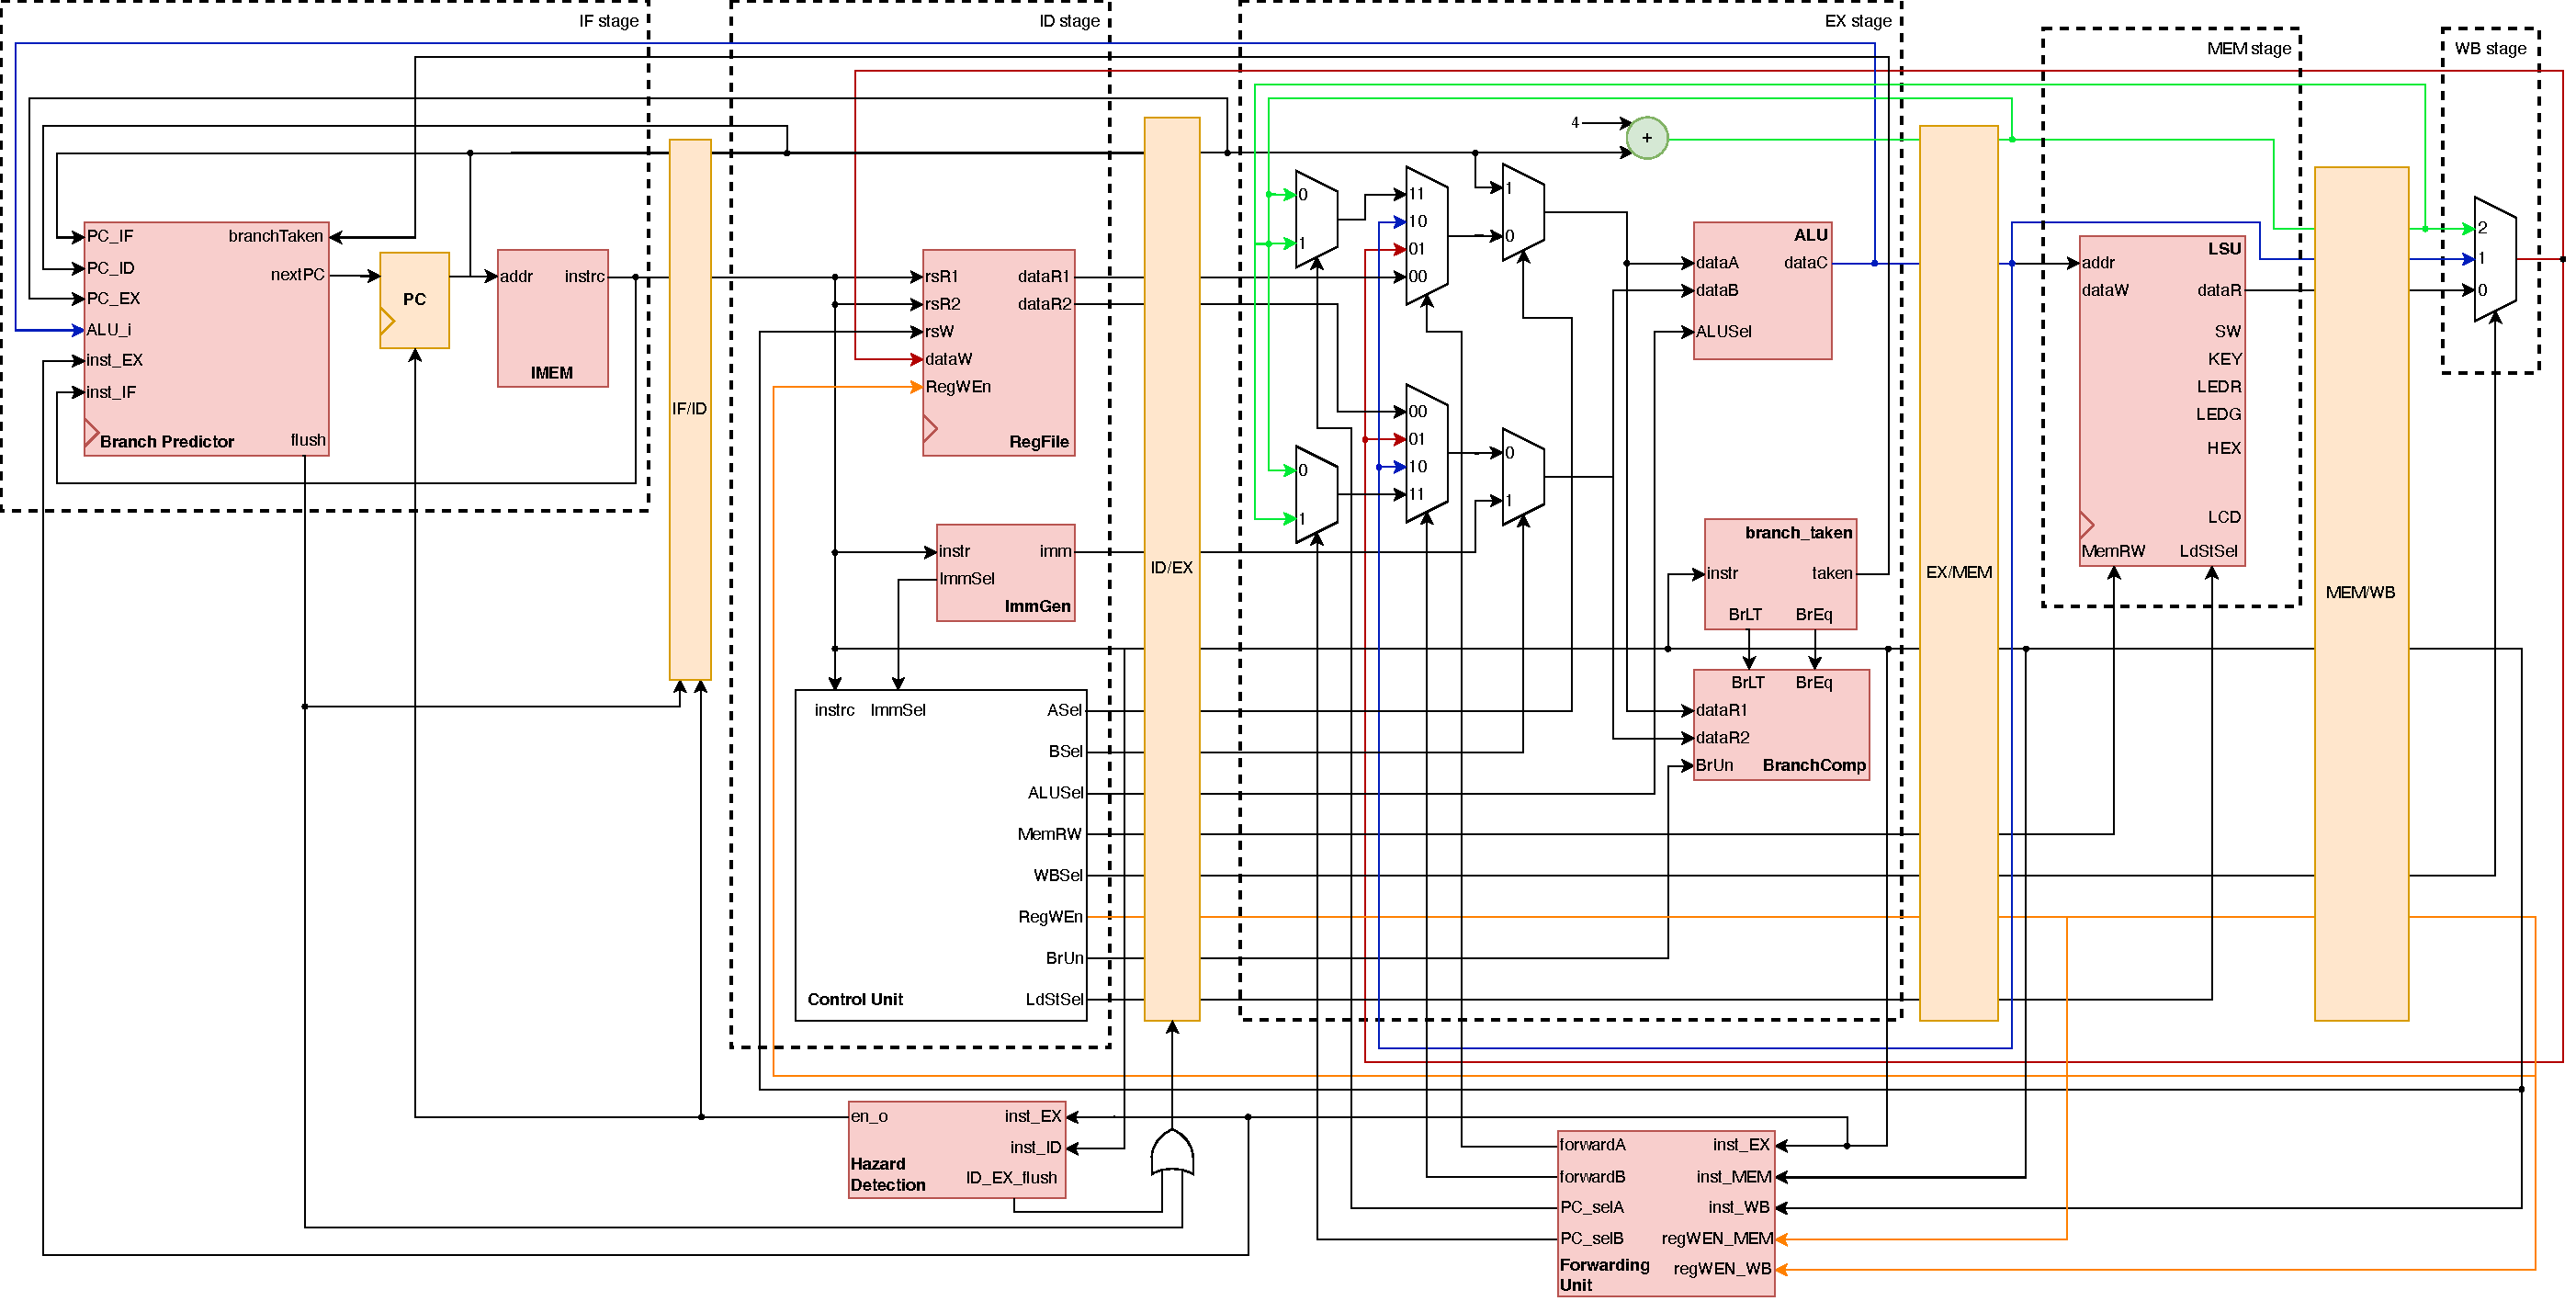
\includegraphics[scale=.5]{images/top_diagram.pdf}
    \caption{Pipelined RV32I Processor Block Diagram}
    \label{top}
\end{figure}
\end{landscape}

\begin{figure}[H]
    \centering
    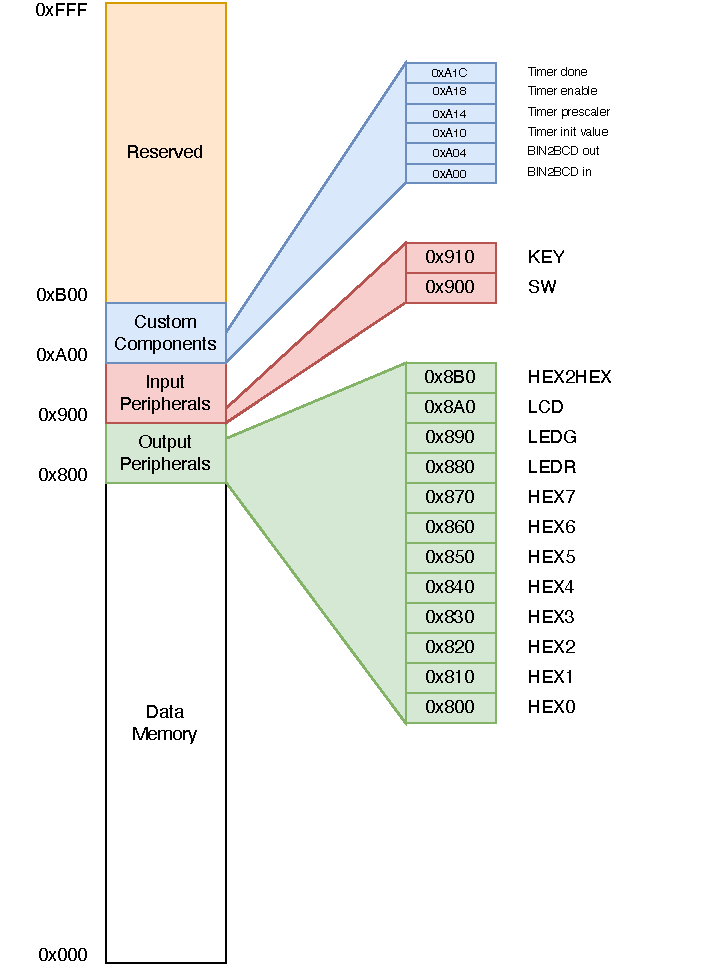
\includegraphics[width=.7\textwidth]{images/memmap.pdf}
    \caption{Updated Memory Mapping Addresses}
\end{figure}


\section{Pipelining}
In this project, we propose a 32-bit integer instruction-based RISC-V processor core. The proposed core has a five-stage pipeline, with proper forwarding and branch prediction. 

\begin{itemize}
    \item In the Instruction Fetch (IF) stage of the pipeline, there incorporates a branch predictor module responsible for branch prediction and an Instruction Memory (IMEM) module for fetching instructions.
    \item Moving to the Instruction Decode (ID) stage, it including the Register File (regfile) module for managing registers, the Immediate Generation (ImmGen) module for generating immediate values, and the Control Logic module for controlling operations.
    \item In Execution (EX) stage, it contains the ALU module, the Branch\_Comp and branch\_taken module. Notably, we add MUX to select the forwarding data.
    \item The Memory (MEM) stage is equipped with the Load-Store Unit (LSU) module, handling data transfer from memory.
    \item Lastly, in the Write-Back (WB) stage, there is a 3-to-1 multiplexer facilitating the selection of the appropriate signal for writing back to the registers.
\end{itemize}

Following the segmentation of a five-stage pipeline, we proceed with the allocation of registers between each stage show on Fig \ref{top}.

\section{Hazards Resolution}
\subsection{RegFile read-after-write data hazard}
The ``read after write''(RAW) hazard in the register file of RISC-V architecture can occur when an instruction tries to read a register immediately after another instruction has written to it.

The solution to mitigate RAW hazards involves implementing the Register File hardware in a way that allows simultaneous read and write operations in different clock edges within the same cycle, which means \textbf{write the register file in the first half of the cycle and read it in the second half}. However, achieving this may not always be feasible, especially in high-frequency designs where timing constraints might limit simultaneous read and write operations.

\subsection{Forwarding Unit}
The Forwarding Unit, also known as a data hazard forwarding unit or simply a forwarding unit, is responsible for forwarding data from the output of one pipeline stage to the input of another, allowing the processor to resolve dependencies and avoid stalls.


The Forwarding Unit module in a processor is designed selecting forwarding data from MEM and WB stages, which is being produced a result that is immediately needed by another instruction in the execution stage, before it's stored in the register file. This bypasses delays caused by waiting for data to be written to the register file, optimizing processing efficiency.
% such as selA, selB, forwardingA, and forwardingB based on the states of the Execution (EX), Memory (MEM), and Write-Back (WB) pipeline stages.

The SystemVerilog code below is describe the forwarding control signal for \texttt{ALU\_A}.
\begin{minted}{sv}
if(regWEn_MEM_i & (rsW_MEM != 5'd0) & (rsW_MEM == rs1_EX)) begin
  if(is_jump_MEM) begin
    forward_sel_A_o   = 2'b11;
    pc_plus_four_selA = 1'b0;
  end else begin
    forward_sel_A_o = 2'b10;
  end
end else if(regWEn_WB_i & (rsW_WB != 5'd0) & (rsW_WB == rs1_EX)) begin
  if(is_jump_WB) begin
    forward_sel_A_o   = 2'b11;
    pc_plus_four_selA = 1'b1;
  end else begin
    forward_sel_A_o = 2'b01;
  end
end
\end{minted}

% The forwarding unit assumes a pivotal role in resolving data hazards within the pipeline, ensuring the seamless execution of instructions. It intervenes in two specific scenarios to modify the pipeline's behavior effectively. Firstly, when an instruction in the Memory (MEM) stage writes to a register and the Execution (EX) stage holds the corresponding result (as denoted by $EX\_MEM\_RegWrite = 1$), the forwarding unit activates the relevant multiplexer (MUX). This activation allows the unit to seamlessly forward the pertinent data, preventing delays and potential hazards. Secondly, when an instruction in the Write-Back (WB) stage writes to a register, and the Memory (MEM) stage contains the value intended for write-back ($MEM\_WB\_RegWrite = 1$), the forwarding unit again engages the appropriate MUX. By intelligently managing these scenarios, the forwarding unit significantly contributes to hazard mitigation, optimizing the pipeline's efficiency and maintaining the accuracy of data flow between different stages.

The Forwarding Unit in RISC-V determines which data to select among Register Data output, ALU result at the MEM stage, data from the write-back MUX, and the PC+4 from either MEM or WB stages, particularly when requiring register data after a \texttt{jal} or \texttt{jalr} instruction. 

\begin{figure}[H]
    \centering
    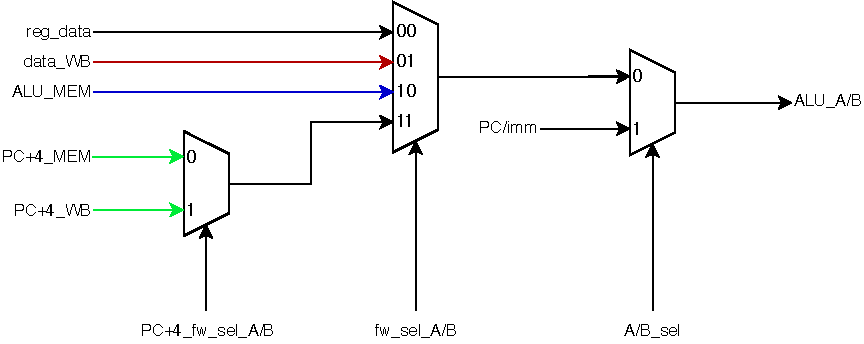
\includegraphics[width=.8\textwidth]{images/fw_sel.pdf}
    \caption{Forwarding Data Selections}
\end{figure}

\subsection{Hazard Detection Unit}
%  In the intricacies of a five-stage pipeline, hazards can impede the seamless execution of instructions. These hazards manifest as structural, data, or control issues. Structural hazards arise when multiple instructions vie for the same hardware resource, necessitating mechanisms to manage resource contention. Data hazards, on the other hand, result from dependencies between instructions concerning the data they manipulate, leading to read-after-write, write-after-read, or write-after-write scenarios. Detecting and resolving data hazards involve techniques such as data forwarding and pipeline stalling. Control hazards come into play when encountering branch instructions, and their resolution often involves predictive mechanisms like branch prediction or speculative execution.
 
% In this module, which receives the Execution (EX) and Instruction Decode (ID) instructions, the focus is on executing processes that trigger flush operations, activate the Program Counter (PC), and enable the Instruction Fetch/Instruction Decode (IF/ID) stage. This execution aims to manage potential hazards, ensuring the proper flow of instructions through the pipeline. By dynamically addressing structural, data, and control issues, this module contributes to the overall efficiency and accuracy of instruction execution in the five-stage pipeline architecture.

The Hazard Detection Unit in a the RISC-V CPU identifies potential hazards that could cause issues in the pipeline and generates control signals to handle them effectively. For instance, in the scenario where the previous \texttt{lw} instruction employs the same destination register as the current \texttt{add} instruction's input register, triggering a hazard, it necessitates the insertion of a \texttt{nop} (no operation) in the pipeline to resolve the conflict and ensure proper execution of instructions without causing errors.

The \texttt{nop} operation is accomplished by disabling the write function for the PC and IF/ID registers, preventing the loading of new instructions. Additionally, flushing the registers in ID/EX is also needed. 

This SystemVerilog code below describe the hazard Detection Unit module.
\begin{minted}{sv}
if(isload_EX & (rsW_EX != 5'd0) & (rsW_EX == rs1_ID | rsW_EX == rs2_ID)) begin
  ID_EX_flush = 1'b1;
  IF_ID_en    = 1'b0;
  pc_en       = 1'b0;
end else begin
  ID_EX_flush = 1'b0;
  IF_ID_en    = 1'b1;
  pc_en       = 1'b1;
end
\end{minted}

\section{Branch Prediction}
\subsection{Branch Target Buffer}

The Branch Target Buffer (BTB) serves as a repository for storing anticipated PC values associated with branch instructions, leveraging the PC itself as an index or address. 

Given that the last two bits of the PC are consistently set to ``\texttt{00}'' utilizing all 30 remaining bits for indexing would lead to an expansive buffer size of $2^{30}$ = 4 gigabytes. This substantial size may prove wasteful, particularly considering that not all instructions within a program are branches. To address this, a refinement is introduced: only the lower bits of the PC are employed as the index, with the remainder designated as tags. And also, the last 2 ``\texttt{00}'' bits are shouldn't be stored in the predicted PC table. This modification seeks to optimize the BTB's storage efficiency, ensuring a more balanced trade-off between memory usage and the imperative for accurate branch prediction in a more compact buffer.

\begin{figure}[H]
    \centering
    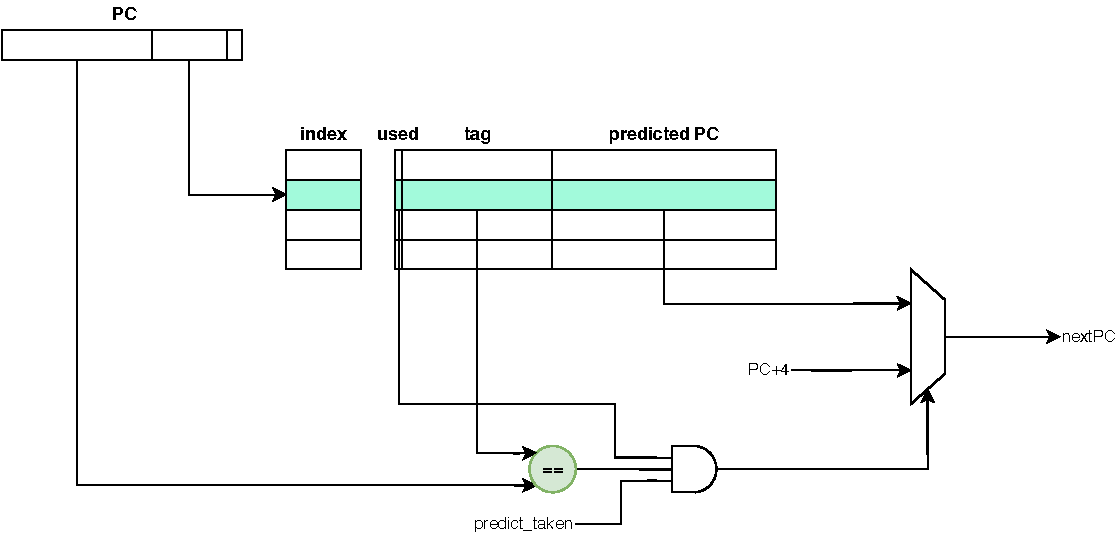
\includegraphics[width=\textwidth]{images/predictor/BTB.pdf}
    \caption{Branch Target Buffer with block diagram}
\end{figure}

Initially, the \texttt{used} flag of the buffer gives 0, indicating no valid entry at that PC index. When a branch instruction is encountered, the processor selects the PC+4 as the default next instruction. As the branch instruction progresses to the EX stage with the determination that the branch is taken, the BTB entry at that index gets updated with new information: the new PC value, the \texttt{tag} (which comprises bits 31 to 20 of the branch PC), and a flag indicating \texttt{used} by setting it to 1. This update ensures the BTB has the most recent and accurate information about branch behavior for future predictions.

\subsection{Predictors}
\subsubsection{Always taken/not taken}

In the context of the RISC-V architecture, "taken" and "not taken" typically refer to the outcomes of branch instructions. Branch Prediction is a technique which predicts the next instruction when the processor faces a branch instruction.

If the branch is always not taken, the processor will always fetch the next instruction at PC+4. In the case of a branch that is always taken, initially, when there's no valid predicted PC in the BTB, the processor does not take the branch and proceeds to fetch the instruction at PC+4. However, if the branch is actually taken, the new PC is updated into the BTB, and subsequent predictions will always take the branch, utilizing the now-valid data in the BTB.

To configure this behavior, setting the \texttt{predict\_taken} signal to a constant value of 0 achieves the ``always not taken'' prediction, ensuring that the processor consistently proceeds with the PC+4 path. Conversely, setting it to a constant value of 1 achieves the ``always taken'' prediction, causing the processor to consistently predict and take branches based on the information stored in the BTB, assuming the branches are always taken.

% \begin{itemize}
%     \item Taken: When a branch instruction is taken, it means that the condition specified in the instruction is met, and the program will jump to a new address or target location.
%     \item Not Taken: When a branch instruction is not taken, it implies that the condition specified in the instruction is not satisfied, and the program continues to execute the next sequential instruction without jumping to a different address.
% \end{itemize}


\subsubsection{n-bit prediction}
\paragraph*{1-bit, 2-bit Predictor}

The 1-bit predictor is the most basic type of dynamic branch predictor. It operates by remembering the direction (taken or not taken) of the last occurrence of a branch instruction and assumes that the same outcome will happen the next time that branch is encountered. It uses a single bit to represent this prediction: \texttt{1} may indicate the branch is taken, and \texttt{0} may suggest the branch is not taken.

\begin{figure}[H]
    \centering
    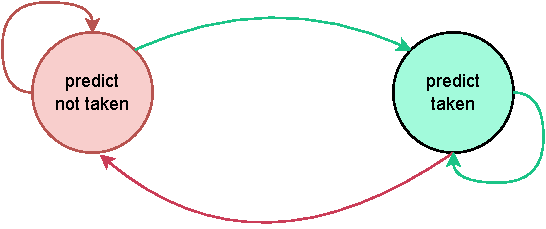
\includegraphics[scale=.90]{images/predictor/taken_not_taken.pdf}
    \caption{1-bit Predictor State Diagram}
\end{figure}

% \begin{figure}[H]
%     \centering
%     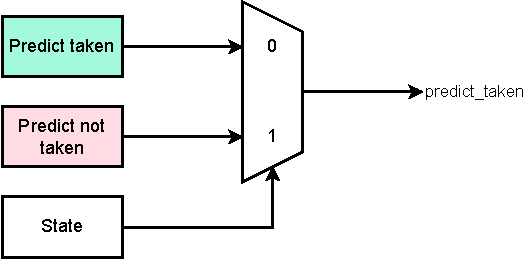
\includegraphics[scale=.90]{images/predictor/1-bit-comb.pdf}
%     \caption{1-bit Predictor with block diagram}
% \end{figure}

Unlike the 1-bit predictor that uses a single bit to represent the prediction, the 2-bit predictor uses two bits per branch. These two bits can represent multiple states of prediction, allowing for a more nuanced approach to track and predict branch behavior. This approach offers better prediction accuracy than a 1-bit predictor because it can capture short-term patterns in branch behavior. It can adapt to changes in the pattern of branches and is less prone to immediate mispredictions caused by occasional deviations from the pattern.

% The two-bit predictor operates within four distinct states, often designated as strongly taken, weakly taken, weakly not taken, and strongly not taken. Specifically, the predictor strongly indicates that the branch will be taken when the two bits are in the state '11'. When the bits are in the '10' state, the predictor foresees the branch being taken but with a diminished level of confidence. In a sequential manner, the predictor indicates that the branch will not be taken but with reduced confidence when the bits are '01'. Finally, when the bits are '00', the predictor anticipates that the branch will not be taken.

% \begin{itemize}
%     \item Strongly Taken: The counter is at its maximum value, indicating a strong tendency for the branch to be taken.

%     \item Weakly Taken: The counter is at a value of 1, suggesting a weaker inclination for the branch to be taken.

%     \item Weakly Not Taken: The counter is at a value of 0, indicating a slight tendency for the branch not to be taken.

%     \item Strongly Not Taken: The counter is at its minimum value, signaling a strong inclination for the branch not to be taken.
% \end{itemize}

\begin{figure}[H]
    \centering
    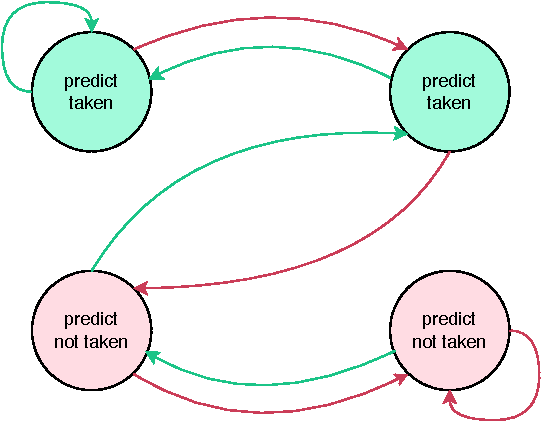
\includegraphics[width=.5\textwidth]{images/predictor/2-bit.pdf}
    \caption{2-bit Predictor State Diagram}
\end{figure}

% \begin{figure}[H]
%     \centering
%     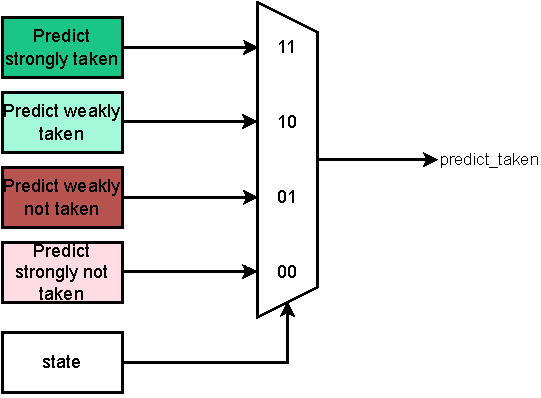
\includegraphics[width=.5\textwidth]{images/predictor/2-bit-comb.pdf}
%     \caption{2-bit Predictor with block diagram}
% \end{figure}

\paragraph*{Saturated Counter}

A/An one/two/n-bit predictor often utilizes a saturated counter as part of its implementation. A saturated counter is a specific type of counter used in branch prediction mechanisms.

A saturated counter is a digital counter with a fixed range of values, and it exhibits a behavior called saturation when it reaches its maximum or minimum limit. The purpose of using a saturated counter is to prevent it from overflowing or underflowing beyond its specified range. This type of counter is commonly employed in various digital systems, including branch predictors in computer architectures. For 1-bit, 2-bit, and n-bit, we use the saturated counter to design and build the module, the MSB of the counter serves as the predict bit.

\begin{figure}[H]
    \centering
    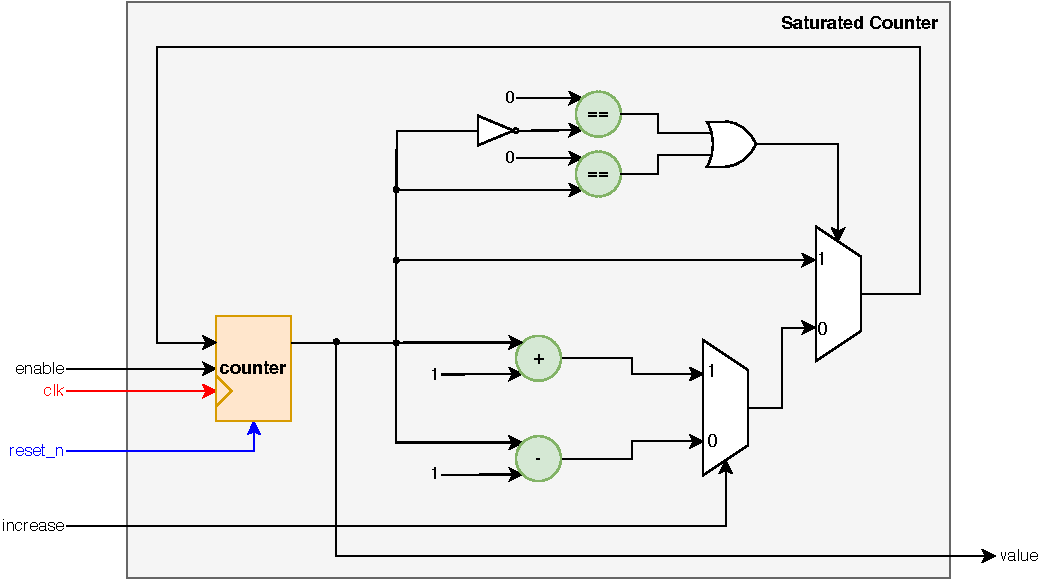
\includegraphics[width=.9\textwidth]{images/predictor/sat_counter.pdf}
    \caption{Saturated Counter Block Diagram}
\end{figure}

\subsubsection{Local prediction}
A local predictor, or PShare, short for ``Per Address Share'', uses an $n$-bit branch PC to index into a Pattern History Table (PHT). This table consists of $2^n$ entries, each storing a $m$-bit taken/not-taken branch history for a specific branch. Subsequently, the $m$-bit pattern history is used to index into Buffer History Table (BHT) with each entry containing a $p$-bit saturating counter, with MSB is the bit to predict taken or not. In this project, we are selecting $n=8$, $m=4$ and $p=2$.

\begin{figure}[H]
    \centering
    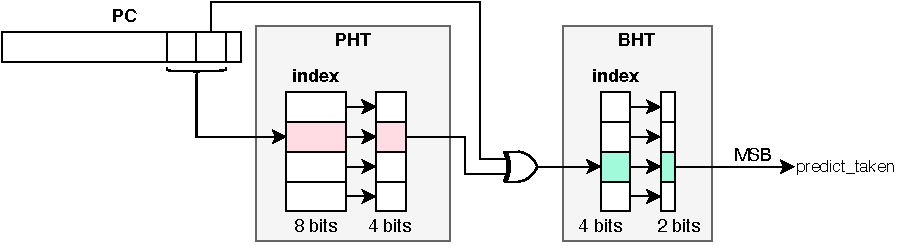
\includegraphics[width=\textwidth]{images/predictor/local.pdf}
    \caption{Local Predictor with block diagram}
\end{figure}

\subsubsection{GShare}
GShare, short for ``Global Share'', is a type of branch predictor used in computer architecture and microprocessor design. It is a hybrid predictor that combines aspects of global history and local history predictors to improve accuracy in predicting the outcome of branch instructions.

\begin{figure}[H]
    \centering
    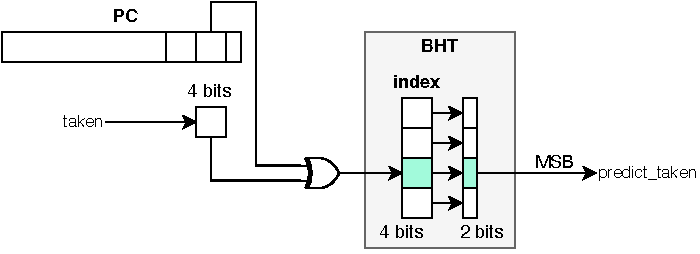
\includegraphics[width=.9\textwidth]{images/predictor/global.pdf}
    \caption{Global Predictor with block diagram}
\end{figure}

\subsubsection{Tournament Prediction}
In tournament predictors, the aim is to combine the strengths of different predictors to create a more robust and accurate prediction mechanism.

This method involves multiple predictors working in parallel, usually a combination of simpler predictors like the local predictor and the global predictor. These predictors compete or against each other to forecast the outcome of a branch instruction.

The tournament predictor often employs a multi-bit counter that keeps track of the performance of different predictors. In this case, an 2-bit saturated counter is utilized where the most significant bit (MSB) of the counter determines the selection between the local and global predictors.

For instance, if the MSB is 0, it indicates a preference for the local predictor, while a value of 1 signifies a preference for the global predictor. The counter increments or decrements based on the accuracy of predictions made by each predictor. When a branch is encountered, the MSB of the counter directs the choice of which predictor to rely on for that specific branch.

This design allows the tournament predictor to dynamically adjust its prediction strategy based on the historical performance of both the local and global predictors, aiming to utilize the most accurate prediction mechanism for improving overall branch prediction accuracy.

\begin{figure}[H]
    \centering
    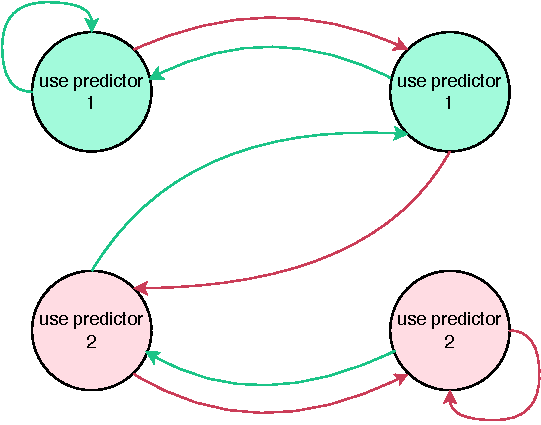
\includegraphics[width=.5\textwidth]{images/predictor/tournament.pdf}
    \caption{Tournament Predictor State Diagram}
\end{figure}

\begin{figure}[H]
    \centering
    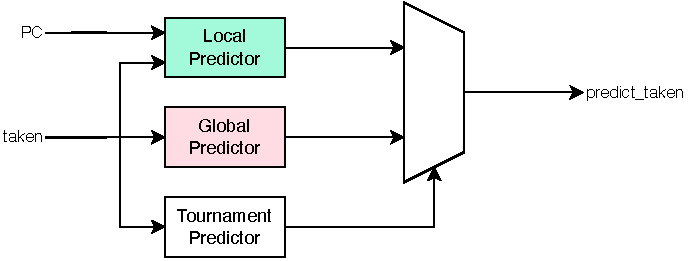
\includegraphics[width=.8\textwidth]{images/predictor/tournament_diagram.pdf}
    \caption{Tournament Predictor with predictors block diagram}
\end{figure}

\chapter{Verification Strategy}
\section{Forwarding Unit}
\subsection{Testcase 1: Forward from MEM and WB stages}
\begin{minted}{asm}
add x5, x3, x2  #
xor x6, x5, x1  # ALU_MEM -> A
sub x9, x3, x5  # WB -> B
or  x2, x7, x5  #
sll x4, x5, x5  #
\end{minted}

\begin{figure}[H]
    \centering
    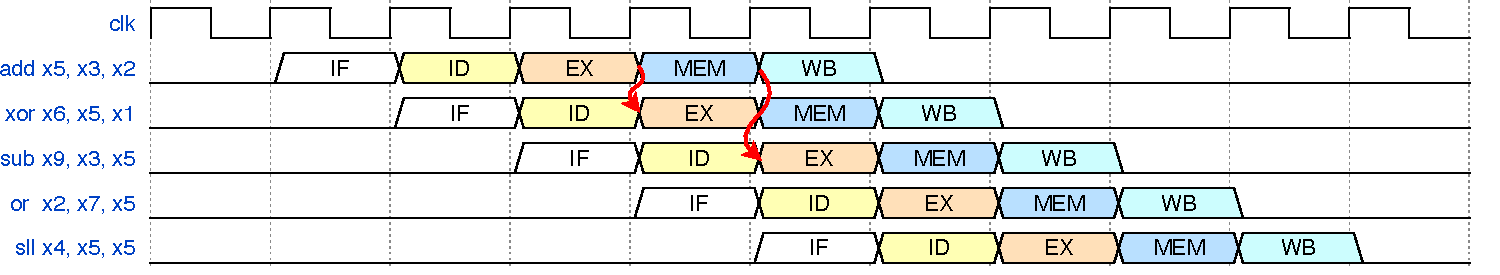
\includegraphics[scale=0.58]{images/tb/fw_case1.pdf}
\end{figure}

\begin{minted}{text}
# Result
inst_EX: 002182b3, ForwardA: 00, ForwardB: 00, PC_fw_A: 0, PC_fw_B: 0
inst_EX: 0012c333, ForwardA: 10, ForwardB: 00, PC_fw_A: 0, PC_fw_B: 0
inst_EX: 405184b3, ForwardA: 00, ForwardB: 01, PC_fw_A: 0, PC_fw_B: 0
inst_EX: 0053e133, ForwardA: 00, ForwardB: 00, PC_fw_A: 0, PC_fw_B: 0
inst_EX: 00529233, ForwardA: 00, ForwardB: 00, PC_fw_A: 0, PC_fw_B: 0
\end{minted}

\subsection{Testcase 2: Forward from MEM and WB stages at the same time}
\begin{minted}{asm}
add x1, x0, x2
add x2, x0, x3
sub x3, x1, x2  # ALU_MEM -> A, WB -> B
\end{minted}

\begin{figure}[H]
    \centering
    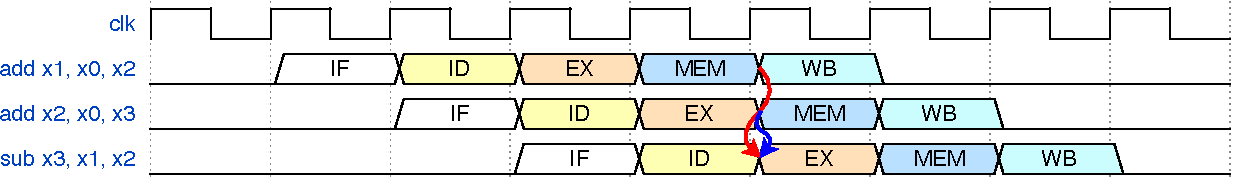
\includegraphics[scale=0.58]{images/tb/fw_case2.pdf}
\end{figure}

\begin{minted}{text}
# Result
inst_EX: 002000b3, ForwardA: 00, ForwardB: 00, PC_fw_A: 0, PC_fw_B: 0
inst_EX: 00300133, ForwardA: 00, ForwardB: 00, PC_fw_A: 0, PC_fw_B: 0
inst_EX: 402081b3, ForwardA: 01, ForwardB: 10, PC_fw_A: 0, PC_fw_B: 0
\end{minted}

\subsection{Testcase 3: Forward PC + 4 from MEM and WB stages}
\begin{minted}{asm}
jal x1, 4
add x2, x1, x0  # pc+4_MEM -> A
add x3, x0, x1  # pc+4_WB -> B
jal x4, 4
jal x5, 8
add x6, x4, x5  # pc+4_WB -> A, pc+4_MEM -> B
\end{minted}

\begin{figure}[H]
    \centering
    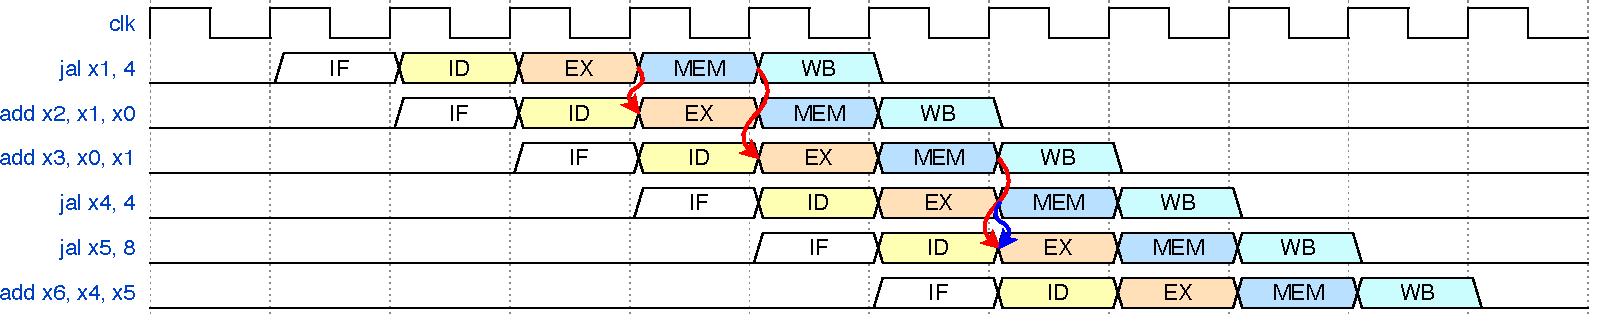
\includegraphics[scale=0.58]{images/tb/fw_case3.pdf}
\end{figure}

\begin{minted}{text}
# Result
inst_EX: 004000ef, ForwardA: 00, ForwardB: 00, PC_fw_A: 0, PC_fw_B: 0
inst_EX: 00008133, ForwardA: 11, ForwardB: 00, PC_fw_A: 0, PC_fw_B: 0
inst_EX: 001001b3, ForwardA: 00, ForwardB: 11, PC_fw_A: 0, PC_fw_B: 1
inst_EX: 0040026f, ForwardA: 00, ForwardB: 00, PC_fw_A: 0, PC_fw_B: 0
inst_EX: 008002ef, ForwardA: 00, ForwardB: 00, PC_fw_A: 0, PC_fw_B: 0
inst_EX: 00520333, ForwardA: 11, ForwardB: 11, PC_fw_A: 1, PC_fw_B: 0
\end{minted}

\section{Hazard Detection Unit}
\subsection{Testcase 1}
\begin{minted}{asm}
add x4, x3, x2
lw  x5, 0x40(x1)
sub x9, x5, x1    # 1 NOP
or  x2, x7, x5
sll x4, x5, x1
\end{minted}

\begin{figure}[H]
    \centering
    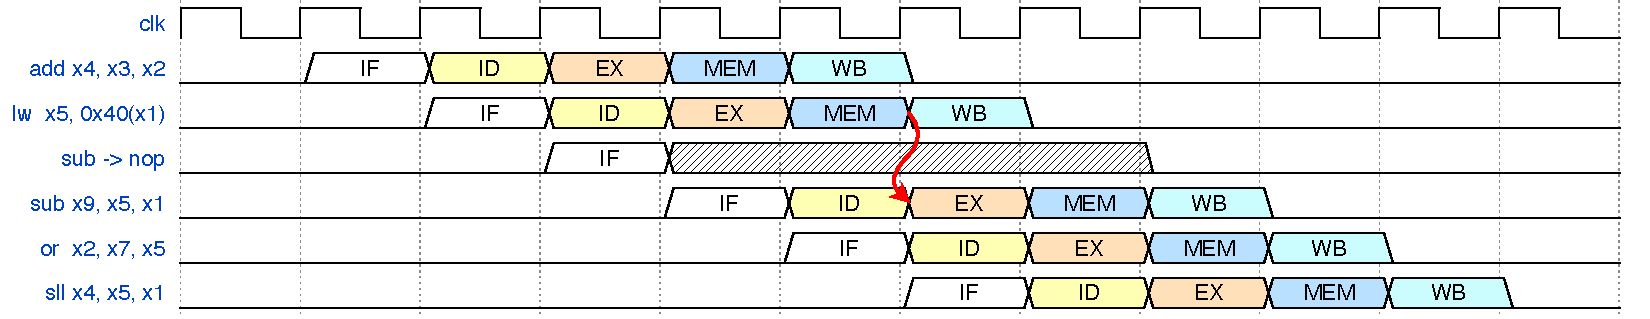
\includegraphics[scale=0.58]{images/tb/hd_case1.pdf}
\end{figure}

\begin{minted}{text}
# Result
inst_EX: 00218233, ID_EX_flush: 0, pc/IF_ID_en: 1
inst_EX: 0400a283, ID_EX_flush: 1, pc/IF_ID_en: 0
inst_EX: 401284b3, ID_EX_flush: 0, pc/IF_ID_en: 1
inst_EX: 0053e133, ID_EX_flush: 0, pc/IF_ID_en: 1
inst_EX: 00129233, ID_EX_flush: 0, pc/IF_ID_en: 1
\end{minted}

\subsection{Testcase 2}
Testcase 2 examines two assembly codes. Testcase 2a intentionally introduces two hazards that require the pipeline to stall for two cycles. Testcase 2b executes the same operations as testcase 2a but in a rearranged assembly codes to avoid creating any stalls.

\subsubsection*{Testcase 2a}
\begin{minted}{asm}
lw x1, 0(x0)
lw x2, 4(x0)
add x3, x1, x2  # 1 NOP
sw x3, 12(x0)
lw x4, 8(x0)
add x5, x1, x4  # 1 NOP
sw x5, 16(x0)
\end{minted}

\begin{figure}[H]
    \centering
    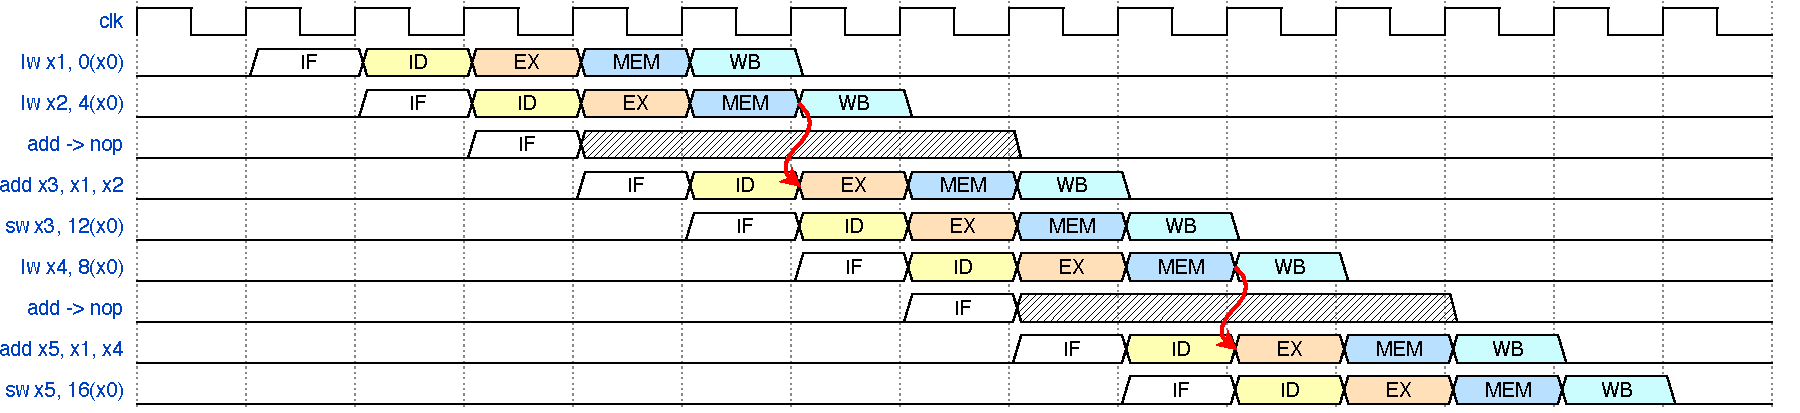
\includegraphics[scale=0.525]{images/tb/hd_case2.pdf}
\end{figure}

\begin{minted}{text}
# Result
inst_EX: 00002083, ID_EX_flush: 0, pc/IF_ID_en: 1
inst_EX: 00402103, ID_EX_flush: 1, pc/IF_ID_en: 0
inst_EX: 002081b3, ID_EX_flush: 0, pc/IF_ID_en: 1
inst_EX: 00302623, ID_EX_flush: 0, pc/IF_ID_en: 1
inst_EX: 00802203, ID_EX_flush: 1, pc/IF_ID_en: 0
inst_EX: 004082b3, ID_EX_flush: 0, pc/IF_ID_en: 1
inst_EX: 00502823, ID_EX_flush: 0, pc/IF_ID_en: 1
\end{minted}

\subsubsection*{Testcase 2b}
\begin{minted}{asm}
lw x1, 0(x0)
lw x2, 4(x0)
lw x4, 8(x0)
add x3, x1, x2  # 0 NOP
sw x3, 12(x0)
add x5, x1, x4  # 0 NOP
sw x5, 16(x0)
\end{minted}

\begin{figure}[H]
    \centering
    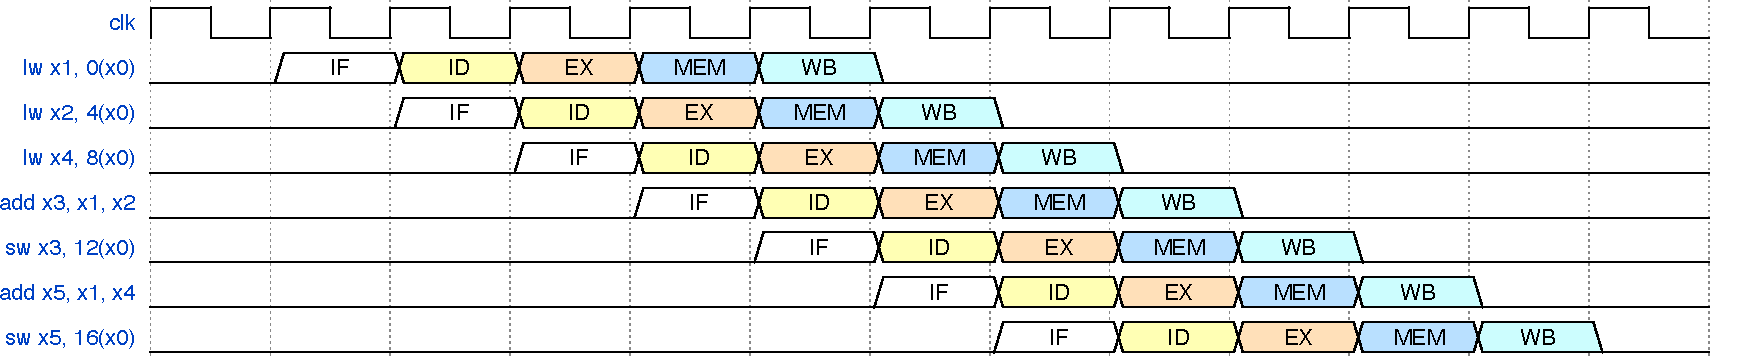
\includegraphics[scale=0.525]{images/tb/hd_case2b.pdf}
\end{figure}

\begin{minted}{text}
# Result
inst_EX: 00002083, ID_EX_flush: 0, pc/IF_ID_en: 1
inst_EX: 00402103, ID_EX_flush: 0, pc/IF_ID_en: 1
inst_EX: 00802203, ID_EX_flush: 0, pc/IF_ID_en: 1
inst_EX: 002081b3, ID_EX_flush: 0, pc/IF_ID_en: 1
inst_EX: 00302623, ID_EX_flush: 0, pc/IF_ID_en: 1
inst_EX: 004082b3, ID_EX_flush: 0, pc/IF_ID_en: 1
inst_EX: 00502823, ID_EX_flush: 0, pc/IF_ID_en: 1
\end{minted}

% \section{Branch predictors}

\section{Run test programs}
The test programs for the single-cycle CPU will be reused to verify. These program will be used for the branch predictors comparison.
\subsection{Factorial Calculation}
\begin{minted}{text}
   0 -- N= 0, expected: 1
 160 --    LEDR output: 1 => PASSED
   0 -- N= 1, expected: 1
 330 --    LEDR output: 1 => PASSED
   0 -- N= 2, expected: 2
 500 --    LEDR output: 2 => PASSED
   0 -- N= 3, expected: 6
 690 --    LEDR output: 6 => PASSED
   0 -- N= 4, expected: 24
 920 --    LEDR output: 24 => PASSED
   0 -- N= 5, expected: 120
1190 --    LEDR output: 120 => PASSED
   0 -- N= 6, expected: 720
1500 --    LEDR output: 720 => PASSED
   0 -- N= 7, expected: 5040
1850 --    LEDR output: 5040 => PASSED
   0 -- N= 8, expected: 40320
2240 --    LEDR output: 40320 => PASSED
   0 -- N= 9, expected: 362880
2670 --    LEDR output: 362880 => PASSED
   0 -- N=10, expected: 3628800
3140 --    LEDR output: 3628800 => PASSED
   0 -- N=11, expected: 39916800
3650 --    LEDR output: 39916800 => PASSED
   0 -- N=12, expected: 479001600
4200 --    LEDR output: 479001600 => PASSED
\end{minted}

\subsection{Fibonacci Sequence Generator}
\label{fibonacci}
\begin{minted}{text}
 160: n =  2, expected =          1, LEDR =          1 => PASSED
 320: n =  3, expected =          2, LEDR =          2 => PASSED
 390: n =  4, expected =          3, LEDR =          3 => PASSED
 460: n =  5, expected =          5, LEDR =          5 => PASSED
 530: n =  6, expected =          8, LEDR =          8 => PASSED
 600: n =  7, expected =         13, LEDR =         13 => PASSED
 670: n =  8, expected =         21, LEDR =         21 => PASSED
 740: n =  9, expected =         34, LEDR =         34 => PASSED
 810: n = 10, expected =         55, LEDR =         55 => PASSED
 880: n = 11, expected =         89, LEDR =         89 => PASSED
 950: n = 12, expected =        144, LEDR =        144 => PASSED
1020: n = 13, expected =        233, LEDR =        233 => PASSED
1090: n = 14, expected =        377, LEDR =        377 => PASSED
1160: n = 15, expected =        610, LEDR =        610 => PASSED
1230: n = 16, expected =        987, LEDR =        987 => PASSED
1300: n = 17, expected =       1597, LEDR =       1597 => PASSED
1370: n = 18, expected =       2584, LEDR =       2584 => PASSED
1440: n = 19, expected =       4181, LEDR =       4181 => PASSED
1510: n = 20, expected =       6765, LEDR =       6765 => PASSED
1580: n = 21, expected =      10946, LEDR =      10946 => PASSED
1650: n = 22, expected =      17711, LEDR =      17711 => PASSED
1720: n = 23, expected =      28657, LEDR =      28657 => PASSED
1790: n = 24, expected =      46368, LEDR =      46368 => PASSED
1860: n = 25, expected =      75025, LEDR =      75025 => PASSED
1930: n = 26, expected =     121393, LEDR =     121393 => PASSED
2000: n = 27, expected =     196418, LEDR =     196418 => PASSED
2070: n = 28, expected =     317811, LEDR =     317811 => PASSED
2140: n = 29, expected =     514229, LEDR =     514229 => PASSED
2210: n = 30, expected =     832040, LEDR =     832040 => PASSED
2280: n = 31, expected =    1346269, LEDR =    1346269 => PASSED
2350: n = 32, expected =    2178309, LEDR =    2178309 => PASSED
2420: n = 33, expected =    3524578, LEDR =    3524578 => PASSED
2490: n = 34, expected =    5702887, LEDR =    5702887 => PASSED
2560: n = 35, expected =    9227465, LEDR =    9227465 => PASSED
2630: n = 36, expected =   14930352, LEDR =   14930352 => PASSED
2700: n = 37, expected =   24157817, LEDR =   24157817 => PASSED
2770: n = 38, expected =   39088169, LEDR =   39088169 => PASSED
2840: n = 39, expected =   63245986, LEDR =   63245986 => PASSED
2910: n = 40, expected =  102334155, LEDR =  102334155 => PASSED
2980: n = 41, expected =  165580141, LEDR =  165580141 => PASSED
3050: n = 42, expected =  267914296, LEDR =  267914296 => PASSED
3120: n = 43, expected =  433494437, LEDR =  433494437 => PASSED
3190: n = 44, expected =  701408733, LEDR =  701408733 => PASSED
3260: n = 45, expected = 1134903170, LEDR = 1134903170 => PASSED
3330: n = 46, expected = 1836311903, LEDR = 1836311903 => PASSED
\end{minted}

\subsection{Find GCD (Great Common Divisor)}

\begin{minted}{text}
A = 48, B = 18, LEDR = 6
A = 92, B = 254, LEDR = 2
A = 68, B = 119, LEDR = 17
\end{minted}

\subsection{Matrix Multiplication}
Evaluate the matrix multiplication, then sum all the value in the result matrix.
$$F=
\left[\begin{matrix}
1 & 2 & 3\\
4 & 5 & 6\\
7 & 8 & 9
\end{matrix}\right]\times
\left[\begin{matrix}
9 & 8 & 7\\
6 & 5 & 4\\
3 & 2 & 1
\end{matrix}\right]=
\left[\begin{matrix}
30 & 24 & 18\\
84 & 69 & 54\\
138 & 114 & 90
\end{matrix}\right]\Rightarrow
\sum F_{ij} = 621
$$

\begin{minted}{text}
LEDR: 621 - Total time spent: 51460
\end{minted}

\subsection{Bubble Sort}
This program will sort an array of 100 pre-defined values stored in data memory (DMEM) using the bubble sort algorithm. Below are the first and last 8 items of both the original and the sorted array.

\begin{minted}{text}
278	 30
33	  31
99	  33
37	  34
338	 35
605	 35
748	 37
238	 52
...         ...
355	 965
223	 978
1001	980
211	 980
66	  991
390	 1000
60	  1001
100	 1009
\end{minted}

All test results have passed, indicating that the program and the CPU are operating correctly.

\chapter{Evaluation}
\section{DE2 Synthesis Evaluation}
\begin{table}[H]
\caption{Maximum Frequency Comparison}
\centering
\begin{tabular}{|l|l|c|}
\hline
\multicolumn{1}{|c|}{\textbf{Predictor Configuration}} & \multicolumn{1}{c|}{$F_{max}$} & \multicolumn{1}{c|}{\textbf{Increased}} \\ \hline
\cellcolor[HTML]{EFEFEF}Single Cycle & \cellcolor[HTML]{EFEFEF}30.44 & \cellcolor[HTML]{EFEFEF}100.00\% \\ \hline
Always Not Taken & 68.66 & 255.56\% \\ \hline
Always Taken & 64.47 & 211.79\% \\ \hline
1-bit Predictor & 65.71 & 215.87\% \\ \hline
2-bit Predictor & 64.19 & 210.87\% \\ \hline
Local Predictor & 64.20 & 210.91\% \\ \hline
Gshare & 64.99 & 213.50\% \\ \hline
Gshare + 2-bit & 65.75 & 216.00\% \\ \hline
Gshare + Local & 64.20 & 210.91\% \\ \hline
\end{tabular}
\end{table}

Based on result from the above table, the pipelined versions achieve a maximum frequency that is more than twice the frequency attained in the single-cycle implementation. The ``Always Not Taken'' model has the highest maximum frequency because there is no need for the BTB, decreasing the length of critical path.

\section{Branch Predictors Evaluation}
\subsection{Pseudo code for loop test cases}
\begin{minted}{C}
// C-Pseudo code for Loop Test 1
int sum = 0;
for(int i = 0; i < 100; i++)
  for(int j = 0; j < 3 ; j++)
    sum += (i-j);
\end{minted}

\begin{minted}{C}
// C-Pseudo code for Loop Test 2
int sum = 0;
for(int i = 0; i < 1000; i++)
  if(i % 2)
    sum += i;
\end{minted}

\subsection{Branch Predictors Comparison}
The ``all branches'' values (``All'' column) represent the total executed branches during program execution. The ``miss'' values (``Miss'' column) signify instances where the ID/EX registers are flushed during execution. Notably, these values pertain specifically to branches and do not include the 2-cycle penalty for jump instructions.

The CPI calculation involves summing the total instructions and adding a 2-cycle penalty for each miss-prediction, then dividing this sum by the total number of instructions, which is $\text{CPI} = \dfrac{\sum \text{instr} + 2\sum \text{br}_{\text{miss}}}{\sum \text{instr} }$.

\begin{table}[H]
\caption{Branch Predictors Comparison}
\centering
\resizebox{\columnwidth}{!}{%
\begin{tabular}{|c||l||r||r|r|r||c|}
\hline
\textbf{Test} & \multicolumn{1}{c||}{\textbf{Predictor}} & \multicolumn{1}{c||}{\textbf{Cycles}} & \multicolumn{1}{c|}{\textbf{Miss}} & \multicolumn{1}{c|}{\textbf{All}} & \multicolumn{1}{c||}{\textbf{Miss Rate}} & \textbf{CPI} \\ \hline\hline
 & \cellcolor[HTML]{EFEFEF}Single Cycle & \cellcolor[HTML]{EFEFEF}20090 & \cellcolor[HTML]{EFEFEF}0 & \cellcolor[HTML]{EFEFEF}501 & \cellcolor[HTML]{EFEFEF}0.000\% & \cellcolor[HTML]{EFEFEF}1.000 \\ \cline{2-7} 
 & Always Not Taken & 22180 & 101 & 501 & 20.160\% & 1.101 \\ \cline{2-7} 
 & Always Taken & 28120 & 398 & 501 & 79.441\% & 1.396 \\ \cline{2-7} 
 & 1-bit Predictor & 24160 & 200 & 501 & 39.920\% & 1.199 \\ \cline{2-7} 
 & 2-bit Predictor & 22180 & 101 & 501 & 20.160\% & 1.101 \\ \cline{2-7} 
 & Local Predictor & 20240 & 4 & 501 & 0.798\% & 1.004 \\ \cline{2-7} 
 & {\color[HTML]{0000FF} Gshare} & {\color[HTML]{0000FF} 20220} & {\color[HTML]{0000FF} 3} & {\color[HTML]{0000FF} 501} & {\color[HTML]{0000FF} 0.599\%} & {\color[HTML]{0000FF} 1.003} \\ \cline{2-7} 
 & {\color[HTML]{0000FF} Gshare + 2-bit} & {\color[HTML]{0000FF} 20220} & {\color[HTML]{0000FF} 3} & {\color[HTML]{0000FF} 501} & {\color[HTML]{0000FF} 0.599\%} & {\color[HTML]{0000FF} 1.003} \\ \cline{2-7} 
\multirow{-9}{*}{\textbf{Loop Test 1}} & {\color[HTML]{0000FF} Gshare + Local} & {\color[HTML]{0000FF} 20220} & {\color[HTML]{0000FF} 3} & {\color[HTML]{0000FF} 501} & {\color[HTML]{0000FF} 0.599\%} & {\color[HTML]{0000FF} 1.003} \\ \hline\hline
 & \cellcolor[HTML]{EFEFEF}Single Cycle & \cellcolor[HTML]{EFEFEF}55080 & \cellcolor[HTML]{EFEFEF}0 & \cellcolor[HTML]{EFEFEF}2001 & \cellcolor[HTML]{EFEFEF}0.000\% & \cellcolor[HTML]{EFEFEF}1.000 \\ \cline{2-7} 
 & Always Not Taken & 65150 & 501 & 2001 & 25.037\% & 1.182 \\ \cline{2-7} 
 & Always Taken & 85130 & 1500 & 2001 & 74.963\% & 1.545 \\ \cline{2-7} 
 & 1-bit Predictor & 75150 & 1001 & 2001 & 50.025\% & 1.363 \\ \cline{2-7} 
 & 2-bit Predictor & 65150 & 501 & 2001 & 25.037\% & 1.182 \\ \cline{2-7} 
 & {\color[HTML]{0000FF} Local Predictor} & {\color[HTML]{0000FF} 55210} & {\color[HTML]{0000FF} 4} & {\color[HTML]{0000FF} 2001} & {\color[HTML]{0000FF} 0.200\%} & {\color[HTML]{0000FF} 1.001} \\ \cline{2-7} 
 & {\color[HTML]{0000FF} Gshare} & {\color[HTML]{0000FF} 55210} & {\color[HTML]{0000FF} 4} & {\color[HTML]{0000FF} 2001} & {\color[HTML]{0000FF} 0.200\%} & {\color[HTML]{0000FF} 1.001} \\ \cline{2-7} 
 & {\color[HTML]{0000FF} Gshare + 2-bit} & {\color[HTML]{0000FF} 55210} & {\color[HTML]{0000FF} 4} & {\color[HTML]{0000FF} 2001} & {\color[HTML]{0000FF} 0.200\%} & {\color[HTML]{0000FF} 1.001} \\ \cline{2-7} 
\multirow{-9}{*}{\textbf{Loop Test 2}} & {\color[HTML]{0000FF} Gshare + Local} & {\color[HTML]{0000FF} 55210} & {\color[HTML]{0000FF} 4} & {\color[HTML]{0000FF} 2001} & {\color[HTML]{0000FF} 0.200\%} & {\color[HTML]{0000FF} 1.001} \\ \hline\hline
 & \cellcolor[HTML]{EFEFEF}Single Cycle & \cellcolor[HTML]{EFEFEF}38170 & \cellcolor[HTML]{EFEFEF}0 & \cellcolor[HTML]{EFEFEF}921 & \cellcolor[HTML]{EFEFEF}0.000\% & \cellcolor[HTML]{EFEFEF}1.000 \\ \cline{2-7} 
 & Always Not Taken & 61530 & 131 & 921 & 14.224\% & 1.069 \\ \cline{2-7} 
 & Always Taken & 54150 & 787 & 921 & 85.451\% & 1.412 \\ \cline{2-7} 
 & 1-bit Predictor & 43190 & 239 & 921 & 25.950\% & 1.125 \\ \cline{2-7} 
 & 2-bit Predictor & 41190 & 139 & 921 & 15.092\% & 1.073 \\ \cline{2-7} 
 & Local Predictor & 41050 & 132 & 921 & 14.332\% & 1.069 \\ \cline{2-7} 
 & Gshare & 41050 & 132 & 921 & 14.332\% & 1.069 \\ \cline{2-7} 
 & Gshare + 2-bit & 41150 & 137 & 921 & 14.875\% & 1.072 \\ \cline{2-7} 
\multirow{-9}{*}{\textbf{\begin{tabular}[c]{@{}c@{}}Factorial\\ (loop \\ 10 times)\end{tabular}}} & {\color[HTML]{0000FF} Gshare + Local} & {\color[HTML]{0000FF} 40890} & {\color[HTML]{0000FF} 124} & {\color[HTML]{0000FF} 921} & {\color[HTML]{0000FF} 13.464\%} & {\color[HTML]{0000FF} 1.065} \\ \hline\hline
 & \cellcolor[HTML]{EFEFEF}Single Cycle & \cellcolor[HTML]{EFEFEF}40220 & \cellcolor[HTML]{EFEFEF}0 & \cellcolor[HTML]{EFEFEF}246 & \cellcolor[HTML]{EFEFEF}0.000\% & \cellcolor[HTML]{EFEFEF}1.000 \\ \cline{2-7} 
 & Always Not Taken & 54000 & 198 & 246 & 80.488\% & 1.098 \\ \cline{2-7} 
 & {\color[HTML]{0000FF} Always Taken} & {\color[HTML]{0000FF} 51160} & {\color[HTML]{0000FF} 56} & {\color[HTML]{0000FF} 246} & {\color[HTML]{0000FF} 22.764\%} & {\color[HTML]{0000FF} 1.028} \\ \cline{2-7} 
 & 1-bit Predictor & 51460 & 71 & 246 & 28.862\% & 1.035 \\ \cline{2-7} 
 & 2-bit Predictor & 51280 & 62 & 246 & 25.203\% & 1.031 \\ \cline{2-7} 
 & Local Predictor & 51540 & 75 & 246 & 30.488\% & 1.037 \\ \cline{2-7} 
 & Gshare & 51460 & 71 & 246 & 28.862\% & 1.035 \\ \cline{2-7} 
 & Gshare + 2-bit & 51400 & 68 & 246 & 27.642\% & 1.034 \\ \cline{2-7} 
\multirow{-9}{*}{\textbf{\begin{tabular}[c]{@{}c@{}}$3\times 3$\\ Matrix\\ Multiplication\end{tabular}}} & Gshare + Local & 51440 & 70 & 246 & 28.455\% & 1.035 \\ \hline\hline
 & \cellcolor[HTML]{EFEFEF}Single Cycle & \cellcolor[HTML]{EFEFEF}6409660 & \cellcolor[HTML]{EFEFEF}0 & \cellcolor[HTML]{EFEFEF}123420 & \cellcolor[HTML]{EFEFEF}0.000\% & \cellcolor[HTML]{EFEFEF}1.000 \\ \cline{2-7} 
 & Always Not Taken & 7277460 & 12583 & 123420 & 10.195\% & 1.039 \\ \cline{2-7} 
 & Always Taken & 9242520 & 110834 & 123420 & 89.802\% & 1.346 \\ \cline{2-7} 
 & 1-bit Predictor & 7519120 & 24665 & 123420 & 19.985\% & 1.077 \\ \cline{2-7} 
 & 2-bit Predictor & 7279460 & 12682 & 123420 & 10.275\% & 1.040 \\ \cline{2-7} 
 & Local Predictor & 7075140 & 2467 & 123420 & 1.999\% & 1.008 \\ \cline{2-7} 
 & Gshare & 7069780 & 2199 & 123420 & 1.782\% & 1.007 \\ \cline{2-7} 
 & Gshare + 2-bit & 7120080 & 4713 & 123420 & 3.819\% & 1.015 \\ \cline{2-7} 
\multirow{-9}{*}{\textbf{Bubble Sort}} & {\color[HTML]{0000FF} Gshare + Local} & {\color[HTML]{0000FF} 7068600} & {\color[HTML]{0000FF} 2140} & {\color[HTML]{0000FF} 123420} & {\color[HTML]{0000FF} 1.734\%} & {\color[HTML]{0000FF} 1.007} \\ \hline
\end{tabular}%
}
\end{table}

In conclusion, simple predictors like Always Taken/Not Taken and 1/2-bit predictors exhibit limitations in adapting to diverse branching patterns, resulting in higher misprediction rates. On the other hand, more sophisticated predictors, especially those incorporating global or local or both, demonstrate improved adaptability and lower misprediction rates. The data emphasizes the importance of history branching patterns for enhancing CPU performance across a range of program complexities, reducing mispredictions, and optimizing the average Cycles Per Instruction (CPI).

\chapter{Conclusion}
This report provides a comprehensive overview of the design and implementation of a pipelined RV32I processor. The processor is meticulously structured into five distinct stages: Instruction Fetch (IF), Instruction Decode (ID), Execute (EX), Memory Access (MEM), and Write Back (WB). Each stage plays a unique role in processing instructions. To address potential data and control hazards during operation, the design incorporates forwarding and hazard detection units.

A notable feature of the processor is the integration of a branch target buffer along with seven diverse branch predictors, including always taken, always not taken, 1-bit, 2-bit, local, GShare, and tournament predictors. These predictors significantly enhance the processor's ability to predict conditional branch instruction outcomes, thereby improving overall efficiency.

To evaluate the processor's functionality and performance, various test programs have been employed, covering operations such as arithmetic operations, loops, and branches. The performance of each branch predictor is assessed using key metrics: miss rate and Cycles Per Instruction (CPI), providing valuable insights into their effectiveness.

Synthesis and implementation of the processor on the DE2 board, a popular FPGA board, have been successfully carried out. The processor achieves maximum frequency of over 60 MHz. This underscores the efficiency of the processor's design and the effectiveness of pipelining.

In conclusion, this project demonstrates the practical feasibility and efficacy of pipelining and branch prediction techniques in enhancing processor efficiency and accuracy. The design and implementation of the pipelined RV32I processor exemplify how these techniques can be applied to create a high-performance processing unit. The insights gained from this report may serve as a valuable guide for future research and development endeavors in the realm of processor design and branch prediction.

\chapter{References}
\nocite{*}
\printbibliography[heading=none]

% \chapter{Source Code}
% \section{\texttt{src/coin\_converter.sv}}
% \inputminted{sv}{source_code/coin_converter.sv}

% \section{\texttt{src/top.sv}}
% \inputminted{sv}{source_code/top.sv}

% \section{\texttt{tb/tb.cpp}}
% \inputminted{cpp}{source_code/tb.cpp}

\end{document}
